%!TEX root = ../report.tex
\begin{document}
\chapter{Methodology}

    % How you are planning to test/compare/evaluate your research.
    % Criteria used.
Dataset bechmarking is important any task because it allows future researchers to compare and validate their methods.
In this thesis, we tried to formulate a benchmark for out of distribution (OOD) detection in 3D datasets and evaluated the benchmarked datasets over the baseline models.
In this chapter, we discuss about the benchmarking of datasets particualry how is it done and experimental setup which includes models used and also a description about the process of OOD detection.

\section{Dataset benchmark formulation}
In this era, development of novel architectures in deep learning is made easy by improvement in frameworks such as Pytorch and Tensorflow. 
These rapidly developed architectures requires a standard benchmarked datasets to compare performance with existing architectures.
The process of creating benchmarked datasets with high quality are tedious and requires Herculian effort. 
Moreover the benchmarking for OOD detection task in 2D is already available in [cite]. 
The benchmarked datasets in OOD detection for 2D classification setting are MNIST vs Fashion MNIST [cite] or CIFAR vs SUN datasets [cite].
Since this thesis deals with OOD detection in 3D segmentation task and it is first of its kind no such benchmarking is available as best of our knowledge.
As discussed in [cite], we chose the datasets for in and out distributions based on the criteria of \textit{relevance}, \textit{representativeness}, \textit{experimentally verified case}, \textit{scalability} and \textit{resuability}.
As argued in [cite] one more criteria is \textit{non-redundancy} was tried to maintain and its only possible with hard OOD scenarios where classes doesn't overlap between datasets. 
In case of soft OOD there are class overlaps but it should not be a problem in OOD detection task.

\subsection{SemanticKITTI}
The first benchmarked datasets are of LiDAR point annotation datasets for 3D semantic segmentation.
This thesis also include the study of the available LiDAR datasets, a detailed descripton of datasets and their classes are availbale in appendix [cite]. 
The discussion here is only confined to the datasets used for benchmarking. 
For this study we chose the SemanticKITTI dataset \cite{Behley_2019_SemanticKITTI} as an in distribution dataset.
We adopted SemanticKITTI becuase of its wide usage in evaluation of 3D semantic segmentation model performance. 
Moreover the dataset consits of high qualitative and quantative scans. 
Also the sensor used is Velodyne HDL-64E which is widely used sensor for LiDAR scans as its used in other datasets such as [cite].
SemanticKITTI \cite{Behley_2019_SemanticKITTI} is a large dataset with 23201 and 20351 scans for training and testing respectively. 
The datasets has a gigantic 4549M number of points which are annotated individually.
It has 28 classes annotated but only 25 are used for evaluation. 
The dataset is also publicly available at [cite] for download and API at [cite].
The available classes and their distribution in dataset is given in Figure \ref{fig:semantic_label_distribution}.
SemanticKITTI is an outdoor autonomous driving dataset as depicted in Figure \ref{fig:semantic_ground_truth_1}.
\begin{figure}[t]
    \centering
    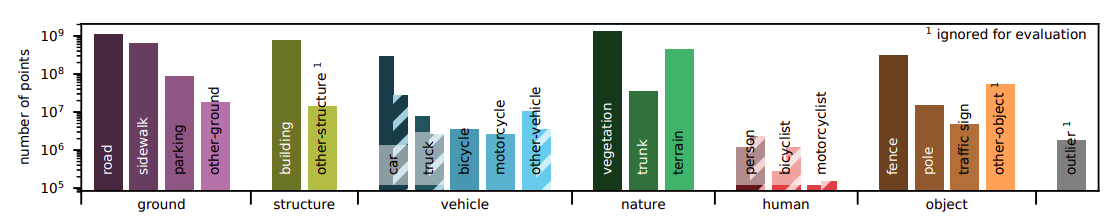
\includegraphics[scale=0.41]{images/semantic_label_distribution.png}
    \caption{Classes in semanticKITTI datset and their distribution in dataset. The hatched bars means a mving object where as solid bar means a non movable object. Image taken from \cite{Behley_2019_SemanticKITTI}.}
    \label{fig:semantic_label_distribution}
\end{figure}
\begin{figure}[t]
    \centering
    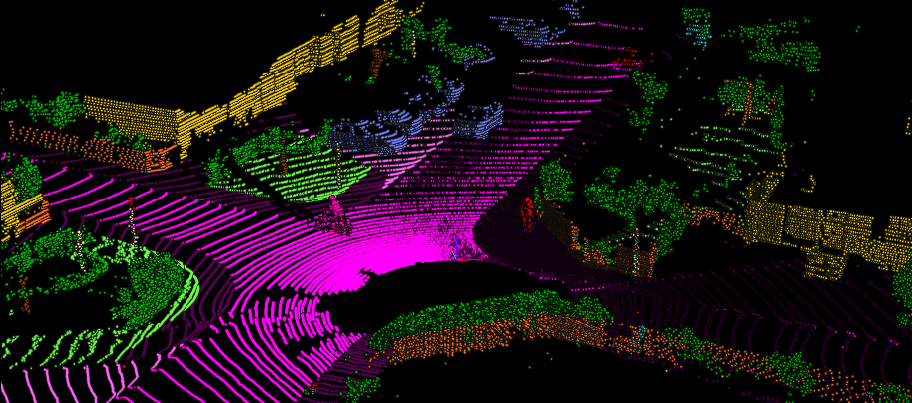
\includegraphics[scale=0.45]{images/semantic_true_label_1.png}
    \caption{Ground truth example of a scan in SemanticKITTI dataset depicting various classes}
    \label{fig:semantic_ground_truth_1}
\end{figure}

\subsection{Stanford 3D Indoor Scene Dataset (S3DIS)}
    % \section{Setup}

    % \section{Experimental Design}
\end{document}
